\documentclass[11pt]{beamer}
%\setbeameroption{show notes}
\usetheme{CambridgeUS}
\usepackage[utf8]{inputenc}
\usepackage[german]{babel}
\usepackage{amsmath}
\usepackage{amsfonts}
\usepackage{amssymb}
\usepackage{url}
%\pgfpageuselayout{4 0n 1 with notes}[a4paper,border shrink=5mm]
\usepackage{color}
\definecolor{mygreen}{rgb}{0,0.6,0}
\definecolor{mygray}{rgb}{0.5,0.5,0.5}
\usepackage{listings}
% https://en.wikibooks.org/wiki/LaTeX/Source_Code_Listings
% http://texblog.org/2012/08/29/changing-the-font-size-in-latex/
\lstset{basicstyle=\scriptsize 
        , commentstyle=\color{mygreen}
        , keywordstyle=\color{blue}
        , language=C++
        %, frame=single
    }

\author{Richard Ulrich}
\title{Trustworthy Software}
\subtitle{Why we sign our binaries and installers}
\setbeamercovered{dynamic} 
\institute{BORM Informatik AG} 
%\date{} 
\subject{BORM developer day} 
\titlegraphic{
\includegraphics[width=2cm]{borm_logo.jpg}}

\begin{document}

%%%%%%%%%%%%%%%%%%%%%%%%%%%%%%%%%%%%%%%%%%%%%%%%%%%%%%%%%%%%%%%%%%%%%%%%%%%%%%%
\begin{frame}
\titlepage
\end{frame}

%%%%%%%%%%%%%%%%%%%%%%%%%%%%%%%%%%%%%%%%%%%%%%%%%%%%%%%%%%%%%%%%%%%%%%%%%%%%%%%
\begin{frame}{Warning when installing PointLine}
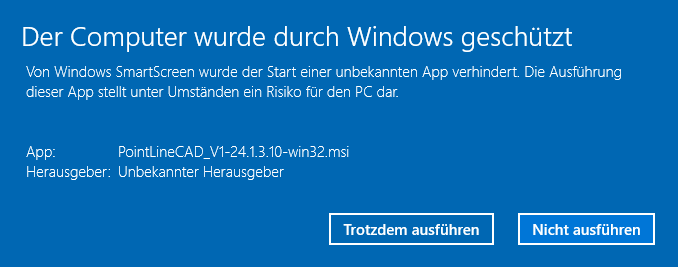
\includegraphics[scale=0.5]{obsolete_signature.png}
\note[itemize]{
\item some of you might have noticed for the first time that we sign our installers when this warning started appearing at the start of 2016 upon trying to install PointLine
\item Who in the audience saw this warning?
\item Who knows why it appeared (except core devs)?
\item We are going to find out in the course of my talk
}
\end{frame}

%%%%%%%%%%%%%%%%%%%%%%%%%%%%%%%%%%%%%%%%%%%%%%%%%%%%%%%%%%%%%%%%%%%%%%%%%%%%%%%
\begin{frame}{Table of contents}
\begin{itemize}
\item How code signing works
\item What the signature asserts
\item What attacks can the signature protect against
\item What attacks does code signing not protect against
\end{itemize}
\end{frame}

%%%%%%%%%%%%%%%%%%%%%%%%%%%%%%%%%%%%%%%%%%%%%%%%%%%%%%%%%%%%%%%%%%%%%%%%%%%%%%%
\begin{frame}{PointLine signature}
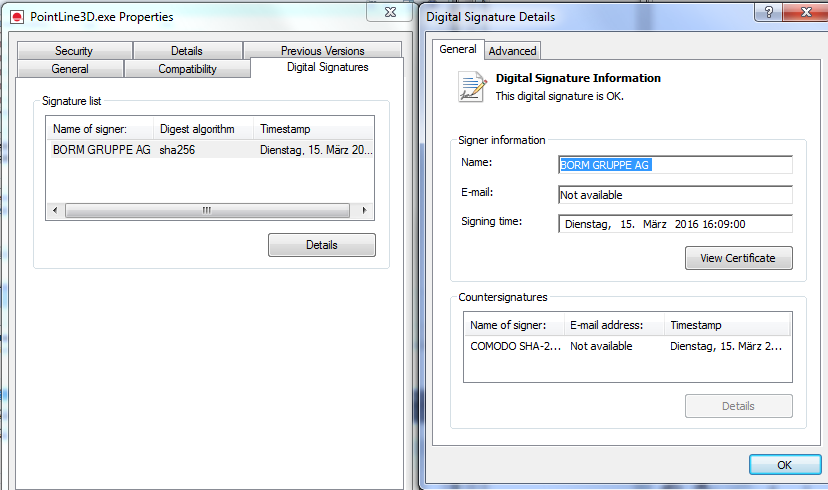
\includegraphics[scale=0.38]{pointLine_signature.png}
\note[itemize]{
\item you can inspect the signature yourself by right-clicking an installer, program file or dll
\item The important part is : This digital signature is OK.
\item The rest is just information, but this means the signature was actually verifyed, 
\item Who in the audience actually checked a signature on an installer or an ISO before installing a software or operating system?
}
\end{frame}

%%%%%%%%%%%%%%%%%%%%%%%%%%%%%%%%%%%%%%%%%%%%%%%%%%%%%%%%%%%%%%%%%%%%%%%%%%%%%%%
\begin{frame}{How code signing works}
\emph{Pre-conditions}
\begin{itemize}
\item Create a large random private key
\item The public key is derived from it
\item Buy a certificate for your public key
\end{itemize}
\pause
\\[0.2cm]
\emph{Signing the software}
\begin{itemize}
\item Create a digest (hash) of the binary
\item Sign it with the private key
\item Signature, public key and certificate are attached to the binary
\end{itemize}
\pause
\\[0.2cm]
\emph{Verifying the signature}
\begin{itemize}
\item Everybody with the public key can verify the signature
\item Certificate creates trust link to known root
\item Roots are shipped with the operating system
\end{itemize}
\note[itemize]{
\item most of this also applies to tls certificates for secure web browsing
}
\end{frame}

%%%%%%%%%%%%%%%%%%%%%%%%%%%%%%%%%%%%%%%%%%%%%%%%%%%%%%%%%%%%%%%%%%%%%%%%%%%%%%%
\begin{frame}{What the signature asserts}
\begin{itemize}
\item Publisher assures that the software is genuine
\item Certificate confirms that the publisher is who he says he is
\item The file did not change since it was signed
\item It was signed on the indicated day (timestamp)
\end{itemize}
\end{frame}

%%%%%%%%%%%%%%%%%%%%%%%%%%%%%%%%%%%%%%%%%%%%%%%%%%%%%%%%%%%%%%%%%%%%%%%%%%%%%%%
\begin{frame}{How do we know the signature is from whom it says}
\begin{itemize}
\item Publisher bought a certificate from a certificate authority
\item The certificate authority checked a trade register document
\item The certificate is signed with the private key of the cert authority
\item The certificate authority bought a certificate from a root authority
\item Root certificates are shipped with the operating system
\end{itemize}
\end{frame}

%%%%%%%%%%%%%%%%%%%%%%%%%%%%%%%%%%%%%%%%%%%%%%%%%%%%%%%%%%%%%%%%%%%%%%%%%%%%%%%
\begin{frame}{Certificate authority hierarchies}
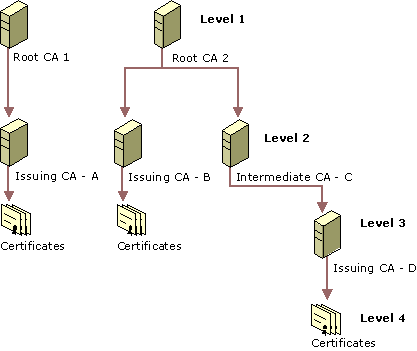
\includegraphics[scale=0.5]{certificate_authority_hierarchies.png}
\end{frame}

%%%%%%%%%%%%%%%%%%%%%%%%%%%%%%%%%%%%%%%%%%%%%%%%%%%%%%%%%%%%%%%%%%%%%%%%%%%%%%%
\begin{frame}{What attacks does the signature protect against}
\begin{itemize}
\item Tampering with the licensing mechanism and selling as original
\item Tampering with the software to make it buggy for discrediting
\item Bundling malware by copycat publisher (angry bird clones)
\item Bundling malware by proxy or man in the middle
\begin{itemize}
\item Internet Service Provider
\item Public, hotel or corporate WiFi
\item TOR exit nodes
\item Great firewall of china
\end{itemize}
\item Bundling malware by download site
\end{itemize}
\end{frame}

%%%%%%%%%%%%%%%%%%%%%%%%%%%%%%%%%%%%%%%%%%%%%%%%%%%%%%%%%%%%%%%%%%%%%%%%%%%%%%%
\begin{frame}{Definition of malware}
\emph{Malware}, short for malicious software, is any software used to disrupt computer operations, gather sensitive information, gain access to private computer systems, or display unwanted advertising.
\\[0.2cm]
\emph{Malware} is defined by its malicious intent, acting against the requirements of the computer user, and does not include software that causes unintentional harm due to some deficiency.
\\[0.1cm]
source: \href{https://en.wikipedia.org/wiki/Malware}{https://en.wikipedia.org/wiki/Malware}
\\[0.5cm]
\pause
My take on the distinction between malware, crapware, bloatware, adware, scareware:\\
\\[0.1cm]
\emph{There no is honor among thieves}\\
\\[0.1cm]
\emph{Ist der Ruf erst ruiniert, lebt es sich ganz ungeniert}
\note[itemize]{
\item If a publisher included adware, how do you know its just that
\item If the unwanted software has a grip on your system, it could grab the more nefarious stuff later on
\item Including unwanted parts, is crossing a line
}
\end{frame}

%%%%%%%%%%%%%%%%%%%%%%%%%%%%%%%%%%%%%%%%%%%%%%%%%%%%%%%%%%%%%%%%%%%%%%%%%%%%%%%
\begin{frame}{definition of backdoor}
A \emph{backdoor} is a method, often secret, of bypassing normal authentication in a product, computer system, cryptosystem or algorithm etc.
\\[0.2cm]
\emph{Backdoors} are often used for securing unauthorized remote access to a computer, or obtaining access to plaintext in cryptographic systems.
\\[0.2cm]
source: \href{https://en.wikipedia.org/wiki/Backdoor\textunderscore(computing)}{https://en.wikipedia.org/wiki/Backdoor\_(computing)}
\end{frame}

%%%%%%%%%%%%%%%%%%%%%%%%%%%%%%%%%%%%%%%%%%%%%%%%%%%%%%%%%%%%%%%%%%%%%%%%%%%%%%%
\begin{frame}{ISP injecting malware}
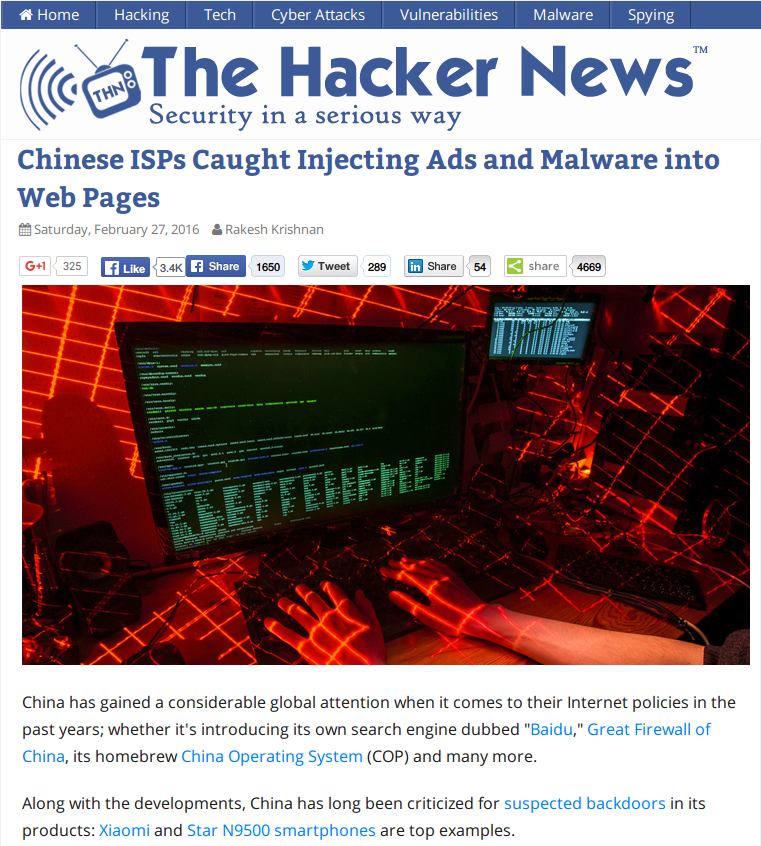
\includegraphics[scale=0.28]{isp_malware.png}
\end{frame}

%%%%%%%%%%%%%%%%%%%%%%%%%%%%%%%%%%%%%%%%%%%%%%%%%%%%%%%%%%%%%%%%%%%%%%%%%%%%%%%
\begin{frame}{Tor exit node tamper windows update}
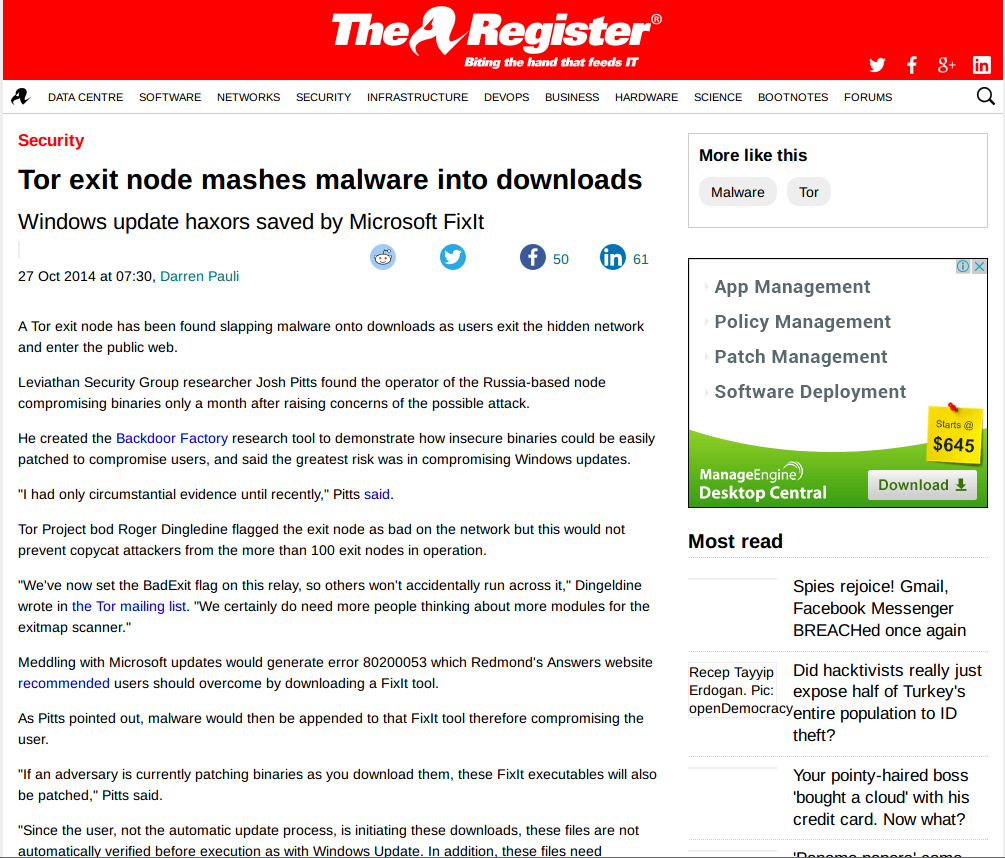
\includegraphics[scale=0.3]{tor_exit_windows_update.png}
\note[itemize]{
\item Compromised windows installer updates detected by signature verification.
\item But the errormessage is unclear, so that the user most likely just continues.
}
\end{frame}

%%%%%%%%%%%%%%%%%%%%%%%%%%%%%%%%%%%%%%%%%%%%%%%%%%%%%%%%%%%%%%%%%%%%%%%%%%%%%%%
\begin{frame}{Injecting JavaScript for distributed denial of service}
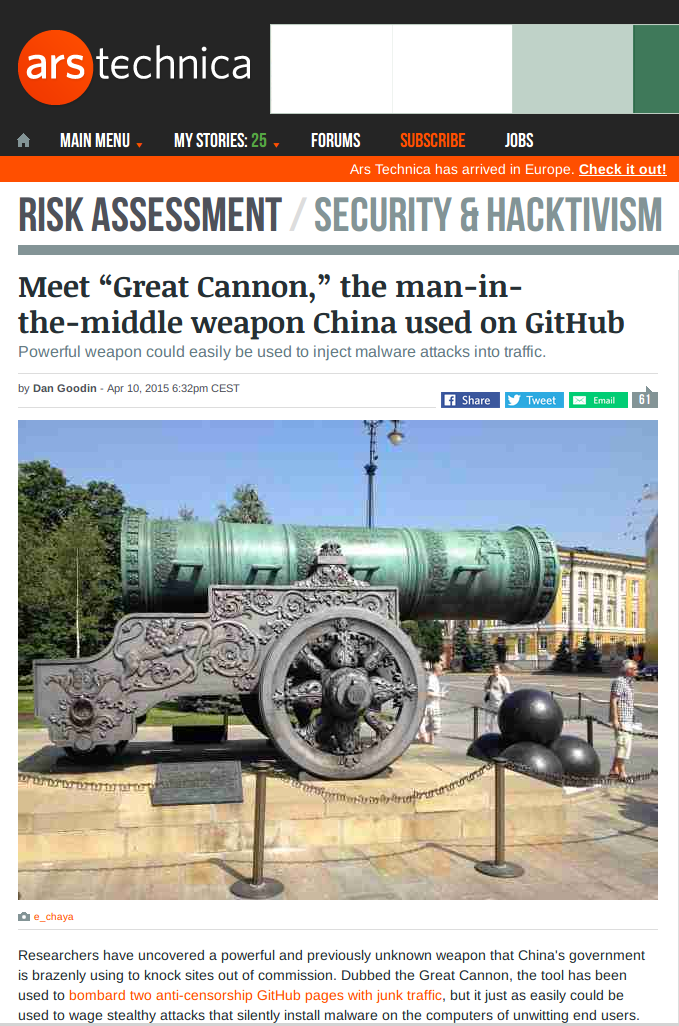
\includegraphics[scale=0.2]{great_canon.png}
\end{frame}

%%%%%%%%%%%%%%%%%%%%%%%%%%%%%%%%%%%%%%%%%%%%%%%%%%%%%%%%%%%%%%%%%%%%%%%%%%%%%%%
\begin{frame}{Involuntarily vulnerable}
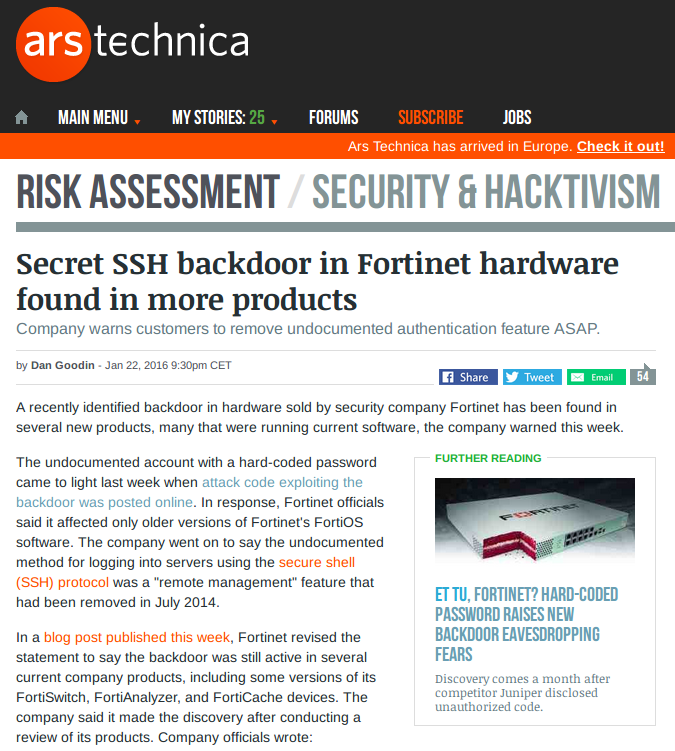
\includegraphics[scale=0.28]{fortinet.png}
\note[itemize]{
\item It doesnt have to be the operator of the network himself
\item A firewall with a known backdoor is an invitation for crooks
\item I think ve have devices from that manufacturer. I hope they were updated.
}
\end{frame}

%%%%%%%%%%%%%%%%%%%%%%%%%%%%%%%%%%%%%%%%%%%%%%%%%%%%%%%%%%%%%%%%%%%%%%%%%%%%%%%
\begin{frame}{SourceForge bundling malware}
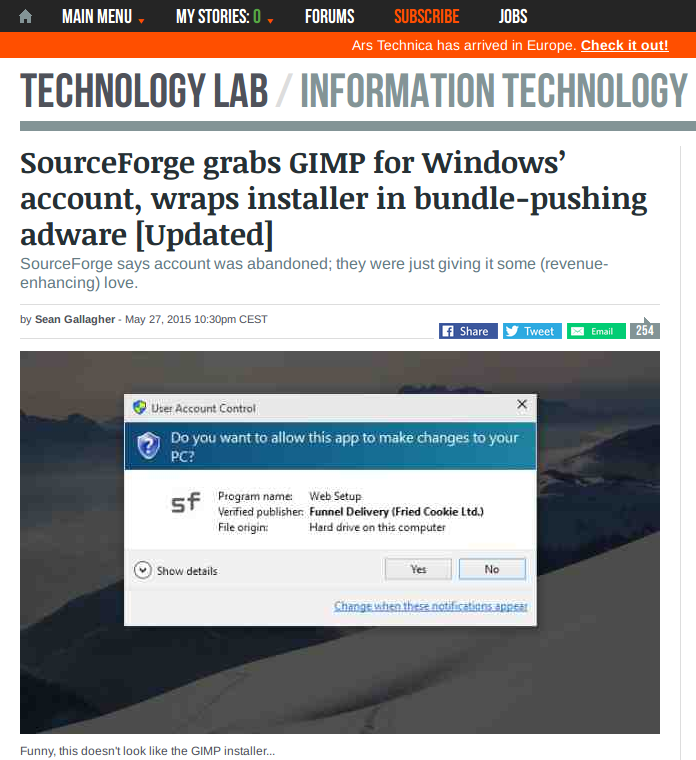
\includegraphics[scale=0.28]{sourceforge.png}
\note[itemize]{
\item Was once the most popular and trusted site to host opensource projects
\item They not only hurt gimp, but completely discredited themselves
\item Is adware less problematic?
\item The screenshot indicates that there is a valid signature, but not from the publisher
}
\end{frame}

%%%%%%%%%%%%%%%%%%%%%%%%%%%%%%%%%%%%%%%%%%%%%%%%%%%%%%%%%%%%%%%%%%%%%%%%%%%%%%%
\begin{frame}{What attacks does code signing not protect against}
\begin{itemize}
\item Weak hash or crypto used for the signature
\item Hacker sneaking backdoor into source code
\item Coerced employee sneaking backdoor into source code
\item Publisher intentionally adding backdoor
\item Compromised build environment (computer)
\item Compromised build tools (compiler)
\item Bundling malware by publisher
\item Insecure coding practices
\item Bribed timestamping provider
\item Compromised certificate authority
\item Private key stolen or unintentionally published
\end{itemize}
\\[0.2cm]
Which of these are targeted vs. automated attacks
\note[itemize]{
\item Lets make a distinction here
\item Hackers select their targets by evaluating return on investment
\item How could we fix these problems?
\item Lets look at them one at a time
}
\end{frame}

%%%%%%%%%%%%%%%%%%%%%%%%%%%%%%%%%%%%%%%%%%%%%%%%%%%%%%%%%%%%%%%%%%%%%%%%%%%%%%%
\begin{frame}{Weak hash or crypto used for the signature}
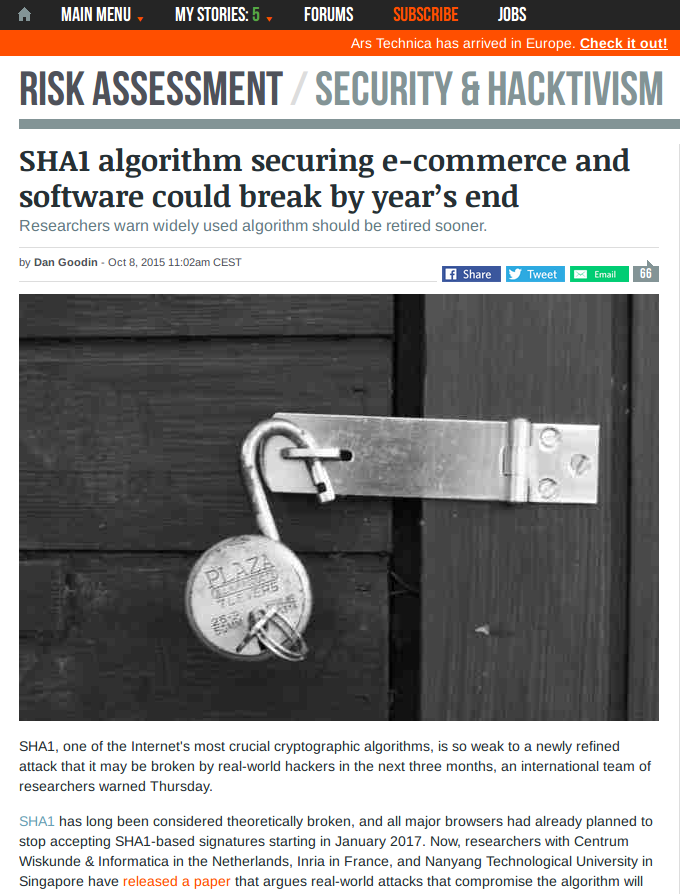
\includegraphics[scale=0.27]{sha1.png}
\note[itemize]{
\item The article is from last october
\item This is what triggered the warning on the first slide
\item It was relatively easy to fix
\item We bought a new certificate and adapted the build process
}
\end{frame}

%%%%%%%%%%%%%%%%%%%%%%%%%%%%%%%%%%%%%%%%%%%%%%%%%%%%%%%%%%%%%%%%%%%%%%%%%%%%%%%
\begin{frame}{Backdoors in the source code}
\emph{Developers can mitigate the risk using:}
\begin{itemize}
\item Good version control system
\item Code reviews
\item Having control over artefacts 
\end{itemize}
\\[0.2cm]
\pause
\emph{But how can the user be confident enough?}
\begin{itemize}
\item Reputation                    
\item Promises                      
\item Independent code reviews      
\item OpenSource                    
\end{itemize}
\note[itemize]{
\item tampering with 3rd party libs might be harder to detect
\item Reputation not enough, but ofthen that s all you get
\item Promises, really? Coerced publisher will deny
\item They are threatened with jail not to disclose
\item Code reviews dont fit well with agile development
\item OpenSource is convincing - the only way you can really trust your software
\item Beleve is for the church. Being able to verify something enables trust.
}
\end{frame}

%%%%%%%%%%%%%%%%%%%%%%%%%%%%%%%%%%%%%%%%%%%%%%%%%%%%%%%%%%%%%%%%%%%%%%%%%%%%%%%
\begin{frame}{Publisher intentionally adding backdoor}
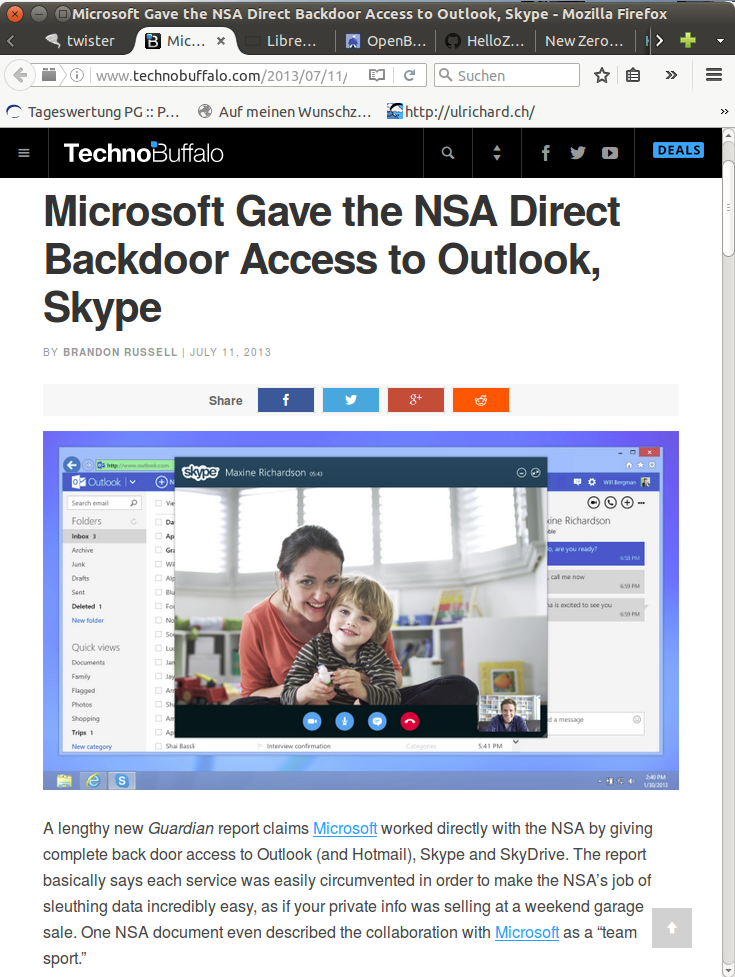
\includegraphics[scale=0.27]{skype.png}
% no big surprise from that company
\end{frame}

%%%%%%%%%%%%%%%%%%%%%%%%%%%%%%%%%%%%%%%%%%%%%%%%%%%%%%%%%%%%%%%%%%%%%%%%%%%%%%%
\begin{frame}{Criminals love backdoors}
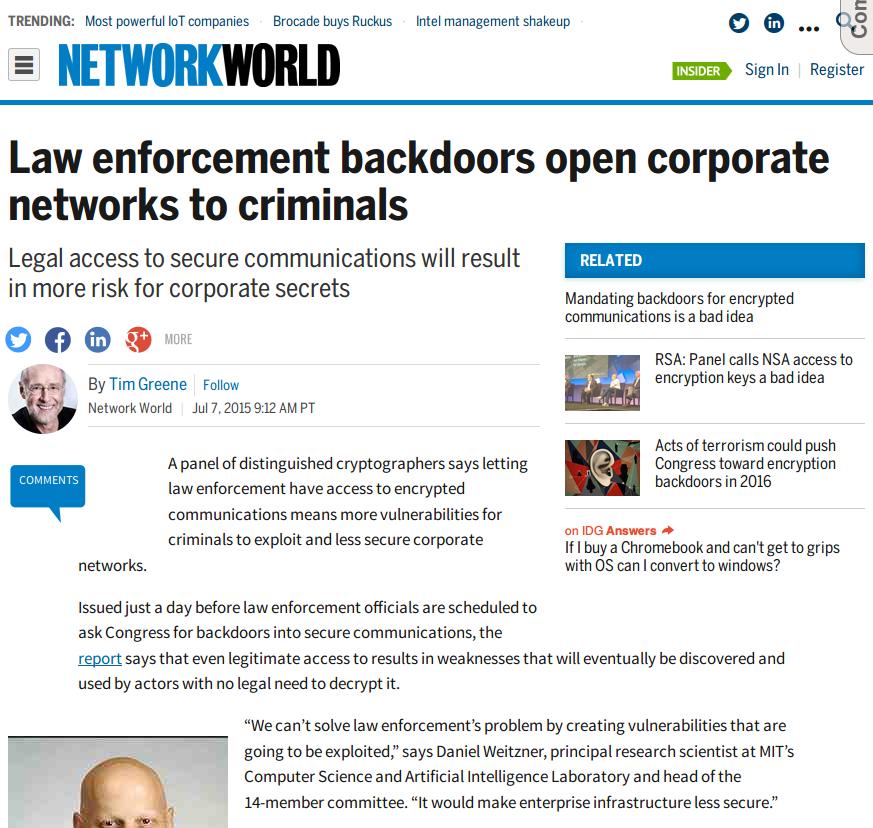
\includegraphics[scale=0.28]{backdoor_criminals.png}
\note[itemize]{
\item the thing with backdoors is that they will be found and used also by criminals
}
\end{frame}

%%%%%%%%%%%%%%%%%%%%%%%%%%%%%%%%%%%%%%%%%%%%%%%%%%%%%%%%%%%%%%%%%%%%%%%%%%%%%%%
\begin{frame}{Once they have access to the network}
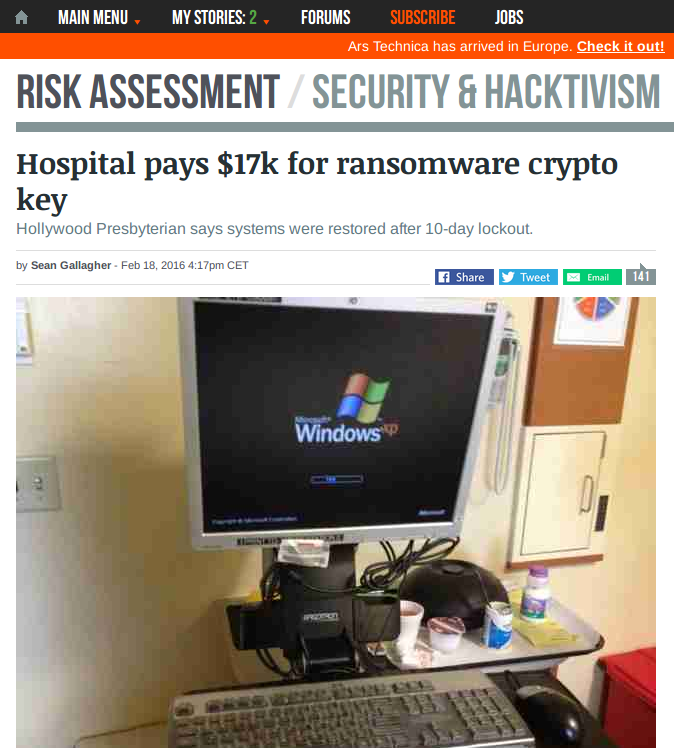
\includegraphics[scale=0.28]{ransomware.png}
\end{frame}

%%%%%%%%%%%%%%%%%%%%%%%%%%%%%%%%%%%%%%%%%%%%%%%%%%%%%%%%%%%%%%%%%%%%%%%%%%%%%%%
\begin{frame}{How small can a backdoor be}
OpenSSH 3.0.2 (CVE-2002-0083)\\
exploitable security bug (privilege escalation: \emph{user can get root}) 
\lstinputlisting[language=C]{@trustworthy_software_SOURCE_DIR@/small_backdoor.c}
\end{frame}

%%%%%%%%%%%%%%%%%%%%%%%%%%%%%%%%%%%%%%%%%%%%%%%%%%%%%%%%%%%%%%%%%%%%%%%%%%%%%%%
\begin{frame}{Resulting difference in the binary}
What is the difference between \textcolor{red}{if (a \textgreater b)} and \textcolor{mygreen}{if (a \textgreater= b)} in x86 assembly? 
\begin{flushleft}
\begin{table}[]
\begin{tabular}{| l | l | l |}
\hline
C        & if (a \textcolor{red}{\textgreater} b) & if (a \textcolor{mygreen}{\textgreater=} b)   \\
assembly & \textcolor{red}{JLE}                   & \textcolor{mygreen}{JL}                       \\
opcode   & 0x7\textcolor{red}{E}                  & 0x7\textcolor{mygreen}{C}                     \\
binary   & 011111\textcolor{red}{1}0              & 011111\textcolor{mygreen}{0}0                 \\
\hline
\end{tabular}
\end{table}
\end{flushleft}
\emph{A single bit!}
\note[itemize]{
\item Does not apply here, but this shows that flipping a single bit in a binary could open a backdoor
\item Luckily if it was flipped later, the signature verification would catch it
}
\end{frame}

%%%%%%%%%%%%%%%%%%%%%%%%%%%%%%%%%%%%%%%%%%%%%%%%%%%%%%%%%%%%%%%%%%%%%%%%%%%%%%%
\begin{frame}{Compromised build environment}
\begin{itemize}
\item Unlikely but very serious\\
\item An attack would have to be targeted\\ % and we are an unlikely target
\item The build host is the one component you still have to trust even with traditional open source distributions. % so far
\end{itemize}
\\[0.2cm]
\pause
\emph{Problems:}
\begin{itemize}
\item Hard to detect
\item Once infected, almost impossible to clean
\item Can result from any backdoored software with enough access
\end{itemize}
\\[0.2cm]
\pause
\emph{What can we do to prevent?}
\begin{itemize}
\item Tight access control and monitoring
\item Redundant build environments  
\item Debian reproducible builds    
\end{itemize}
\note[itemize]{
\item Redundant systems alone are not enough
\item Builds are usually not binary equal. Even timestamps can make the difference
\item Reproducible builds close the last loophole
}
\end{frame}

%%%%%%%%%%%%%%%%%%%%%%%%%%%%%%%%%%%%%%%%%%%%%%%%%%%%%%%%%%%%%%%%%%%%%%%%%%%%%%%
\begin{frame}{Motivation for reproducible builds}
With free software, anyone can inspect the source code for malicious flaws. But Debian provide binary packages to its users. The idea of “deterministic” or “reproducible” builds is to empower anyone to verify that no flaws have been introduced during the build process by reproducing byte-for-byte identical binary packages from a given source. \\
source: \href{https://wiki.debian.org/ReproducibleBuilds/About}{https://wiki.debian.org/ReproducibleBuilds/About}
\\[0.1cm]
We often speak as if open source software can't contain backdoors or malware because its source code is "published", rendering any potentially malicious code visible. But real-world software release processes have major transparency gaps that aren't addressed by most existing open source development practices. The biggest such gap is that compilation and packaging processes aren't reproducible. Trying to recreate these processes typically yields a different result. That means users can't directly verify that the binary releases they download and use were actually created from the purportedly corresponding source trees.\\
source: \href{https://air.mozilla.org/why-and-how-of-reproducible-builds-distrusting-our-own-infrastructure-for-safer-software-releases/}{https://air.mozilla.org/why-and-how-of-reproducible-builds-distrusting-our-own-infrastructure-for-safer-software-releases/}
\note[itemize]{
\item read only the debian part
}
\end{frame}

%%%%%%%%%%%%%%%%%%%%%%%%%%%%%%%%%%%%%%%%%%%%%%%%%%%%%%%%%%%%%%%%%%%%%%%%%%%%%%%
\begin{frame}{Debian build procedure}
\begin{itemize}
\item Upstream author releases a source tarball with signature
\pause
\item Debian developer creates a source package which:
\begin{itemize}
\item Specifies where the original sources and signature can be downloaded
\item Specifies how the package is built
\item Might add some debian specific patches
\item Includes the public key of the upstream author in the package
\item Signs the source package and uploads it to the repository
\end{itemize}
\pause
\item Build servers:
\begin{itemize}
\item Download the source package and the original tarbal
\item Verify both signatures
\item Apply the patches
\item Build as instructed
\item Create a binary package
\item Sign the binary package and uploads it to the repository
\end{itemize}
\pause
\item Binary packages from multiple build servers are compared
\item Currently 87.6\% of debian packages build reproducibly for amd64
\end{itemize}
\note[itemize]{
\item For the current stable release there were other priorities, but it will be one of the big points for the next one.
\item Imagine how much harder it would be for VW to roll out cheating emission controls with a process like this
}
\end{frame}

%%%%%%%%%%%%%%%%%%%%%%%%%%%%%%%%%%%%%%%%%%%%%%%%%%%%%%%%%%%%%%%%%%%%%%%%%%%%%%%
\begin{frame}{Package overview}
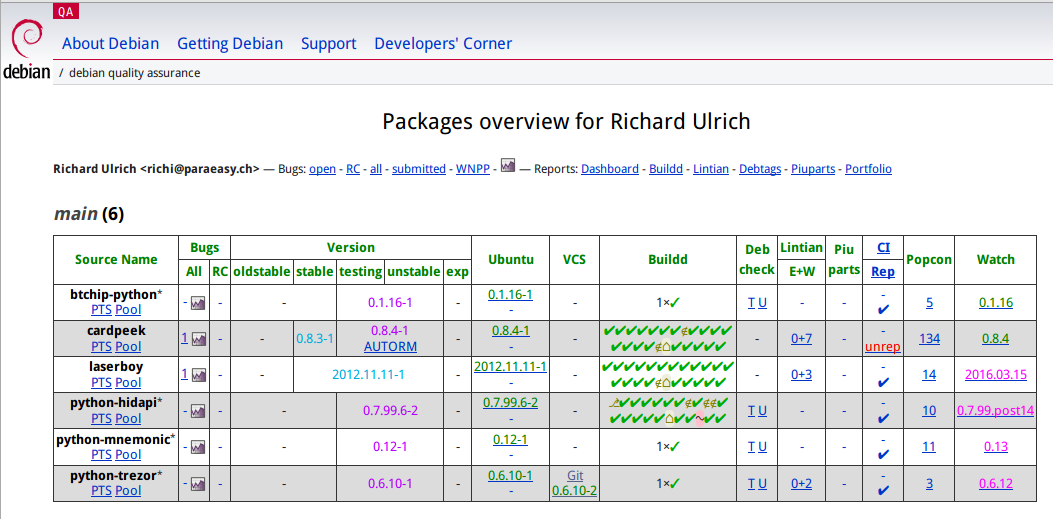
\includegraphics[scale=0.33]{debian_qa.png}
\note[itemize]{
\item cardpeek has a reproducibility problem
\item some packages don't build on esotheric or experimental platforms such as ppc, hurd or kfreebsd
\item architecture independent packages have only 1 check mark. Python packages for example are shipped with the sources, and only as a post install step are the pyc files created on the target machine.
}
\end{frame}

%%%%%%%%%%%%%%%%%%%%%%%%%%%%%%%%%%%%%%%%%%%%%%%%%%%%%%%%%%%%%%%%%%%%%%%%%%%%%%%
\begin{frame}{Compromised build tools}
\emph{Unlikely but very serious}
\\[0.2cm]
\begin{itemize}
\item Not much you can do
\item Trust whomever sold it to you
\item Use a well reviewed open source tool chain
\end{itemize}
\note[itemize]{
\item hard to defend against
}
\end{frame}

%%%%%%%%%%%%%%%%%%%%%%%%%%%%%%%%%%%%%%%%%%%%%%%%%%%%%%%%%%%%%%%%%%%%%%%%%%%%%%%
\begin{frame}{This is not just theory}
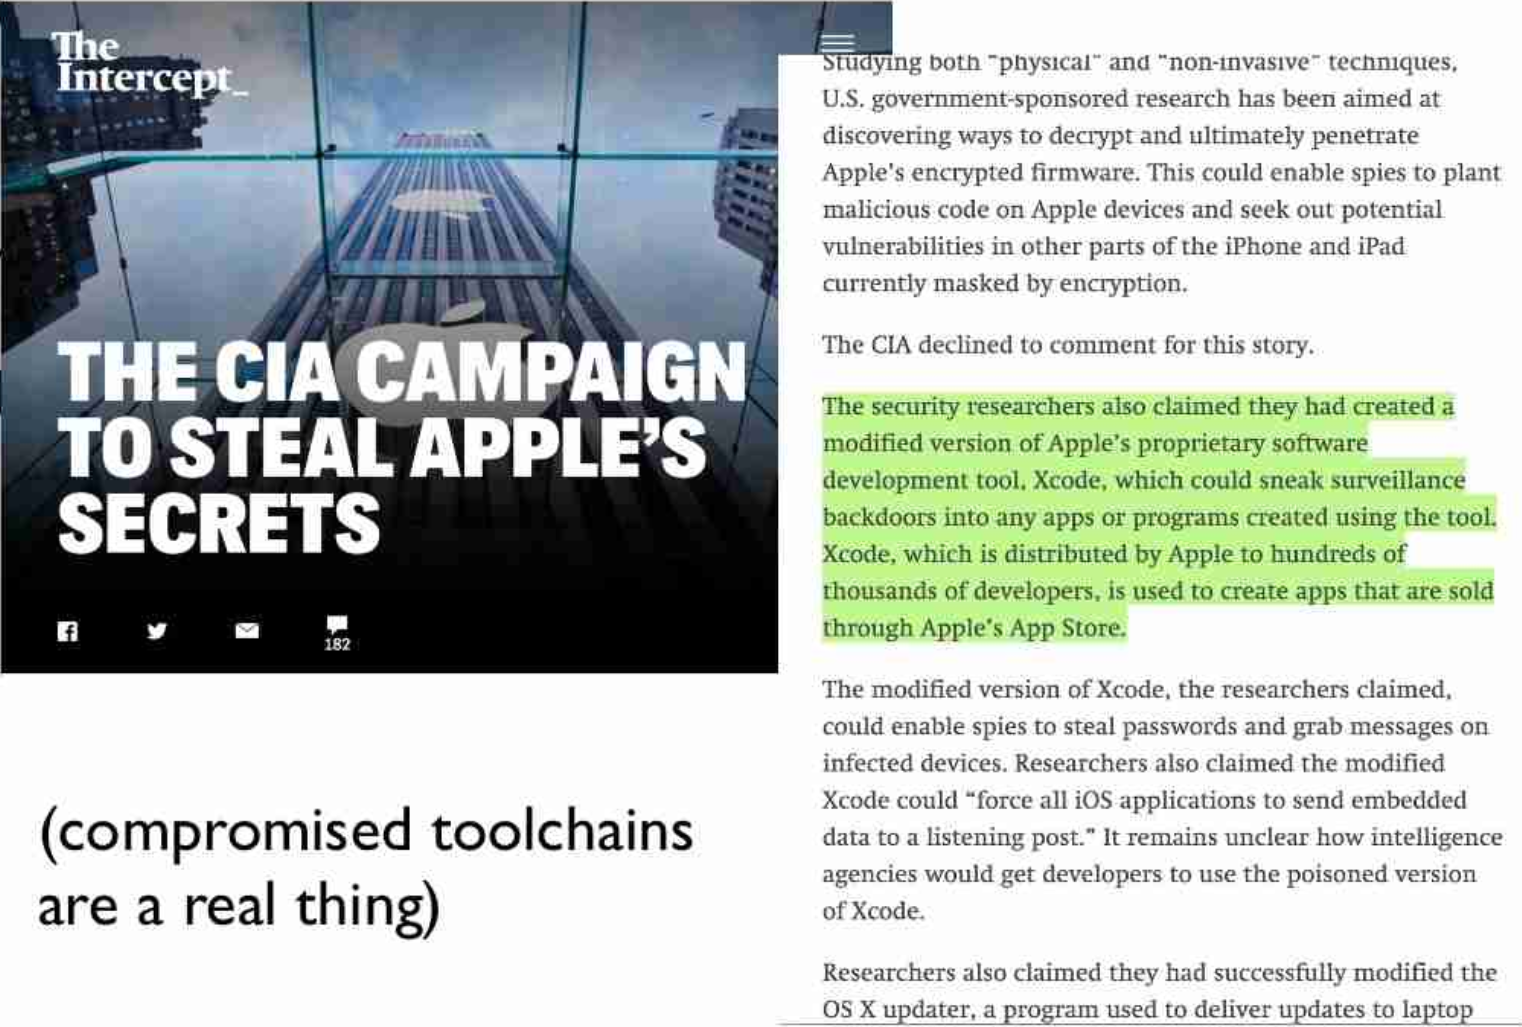
\includegraphics[scale=0.23]{apple_toolchain.png}
\end{frame}

%%%%%%%%%%%%%%%%%%%%%%%%%%%%%%%%%%%%%%%%%%%%%%%%%%%%%%%%%%%%%%%%%%%%%%%%%%%%%%%
\begin{frame}{Bundling malware by publisher}
\emph{Examples:}
\begin{itemize}
\item Oracle Java
\item Compression tool served by Npackd % a package manager for windows
\item Email offers if you ever published an Android app
\end{itemize}
\\[0.2cm]
\pause
\emph{As a software publisher:}
\begin{itemize}
\item Just don't do it!
\item Loosing users and trust is not worth the few bucks
\end{itemize}
\\[0.2cm]
\pause
\emph{As the user:}
\begin{itemize}
\item Why a \emph{singing santa} app wants access to your private data?
\item I try to avoid software, if I have reason to beleve it is compromised % even if it is forced on us
\begin{itemize}
\item Or if the company uses other abusive practices such as
\begin{itemize}
\item Bribing or deception
\item Vendor-lock-in
\item Digital Rights Management
\end{itemize}
\end{itemize}
\item There are always plenty of good alternatives
\end{itemize}
\end{frame}

%%%%%%%%%%%%%%%%%%%%%%%%%%%%%%%%%%%%%%%%%%%%%%%%%%%%%%%%%%%%%%%%%%%%%%%%%%%%%%%
\begin{frame}{Bundling malware by publisher}
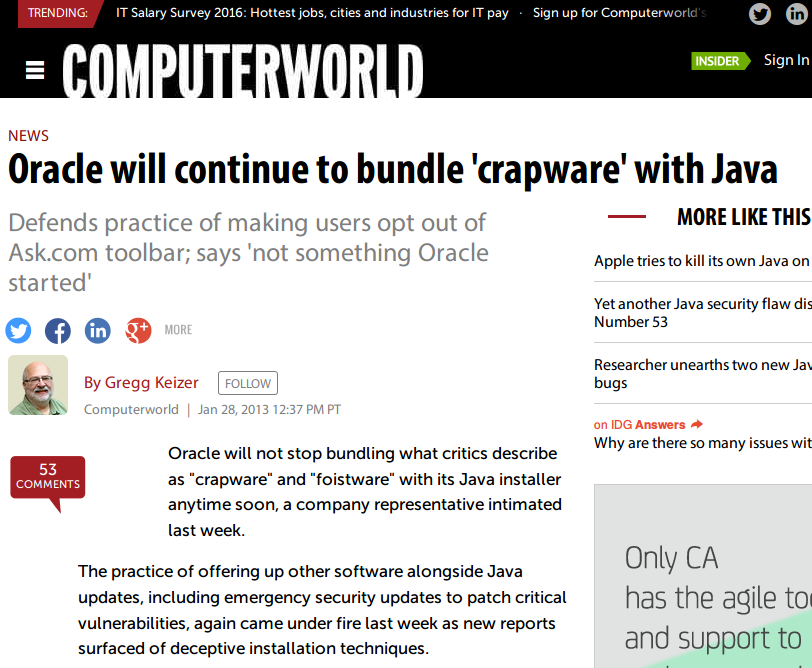
\includegraphics[scale=0.3]{oracle.png}
\end{frame}

%%%%%%%%%%%%%%%%%%%%%%%%%%%%%%%%%%%%%%%%%%%%%%%%%%%%%%%%%%%%%%%%%%%%%%%%%%%%%%%
\begin{frame}{Insecure coding practices}
\emph{As a software publisher:}
\begin{itemize}
\item I won't go into details here
\item Events just like today address this very issue
\end{itemize}
\\[0.2cm]
\pause
\emph{As the user:}
\begin{itemize}
\item With closed source software, you can only guess
\item A shiny GUI tells nothing about what's behind
\item If it crashes a lot, there might be more at odds
\end{itemize}
\end{frame}

%%%%%%%%%%%%%%%%%%%%%%%%%%%%%%%%%%%%%%%%%%%%%%%%%%%%%%%%%%%%%%%%%%%%%%%%%%%%%%%
\begin{frame}{Bribed timestamping provider}
This is probably the least severe case here
\\[0.2cm]
Timestamp provider is a single point of failure.
\\[0.2cm]
More secure methods, you can prove something existed at a certain date.
\\[0.2cm]
\pause
\begin{itemize}
\item Create a hash of a document and publish it in a newspaper
\pause
\item There is a service called \emph{proof of existence} that stores the hash on the BitCoin blockchain
\end{itemize}
\note[itemize]{
\item Nobody would even care if PointLine had a wrong timestamp in the signature.
\item The warning on the first slide could be avoided with a 2015 timestamp.
\item But it's much easier to buy a new certificate.
\item Ideas from the audience for more secure methods?
\item BitCoin's BlockChain is a tamper resistant distributed consensus system
}
\end{frame}

%%%%%%%%%%%%%%%%%%%%%%%%%%%%%%%%%%%%%%%%%%%%%%%%%%%%%%%%%%%%%%%%%%%%%%%%%%%%%%%
\begin{frame}{Compromised certificate authority}
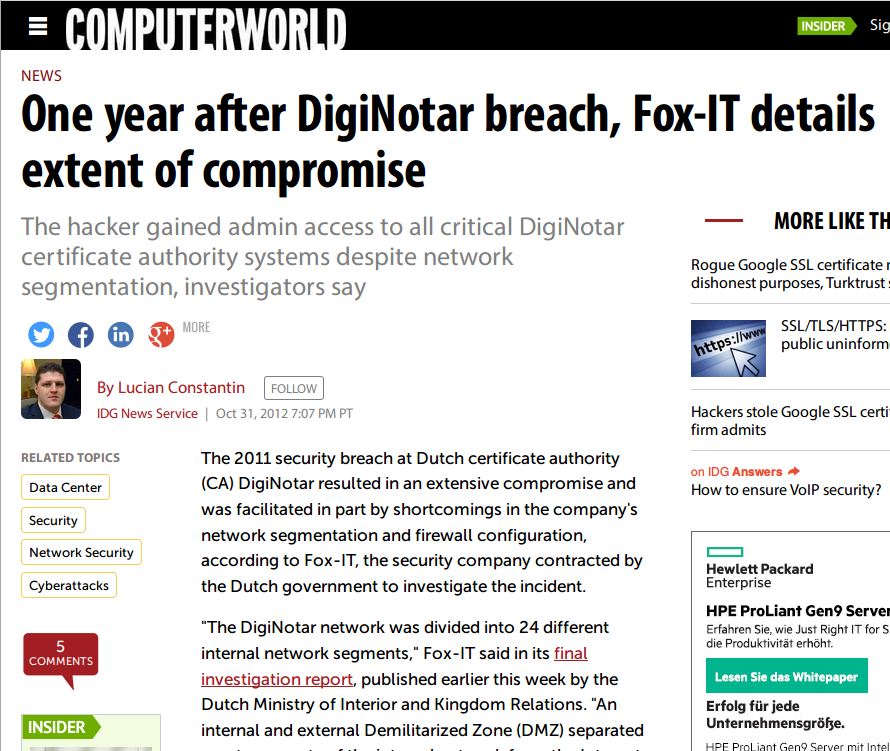
\includegraphics[scale=0.28]{diginotar.png}
\end{frame}

%%%%%%%%%%%%%%%%%%%%%%%%%%%%%%%%%%%%%%%%%%%%%%%%%%%%%%%%%%%%%%%%%%%%%%%%%%%%%%%
\begin{frame}{Compromised certificate authority}
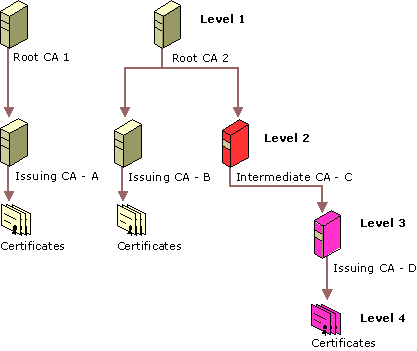
\includegraphics[scale=0.5]{certificate_authority_compromised.png}
\note[itemize]{
\item First the compromise has to be noticed
\item Revoking the key invalidates also lots of legitimate certificates
\item Timestamps could play a more important role here
\item Why do we have such a hierarchical structure in the first place?
}
\end{frame}

%%%%%%%%%%%%%%%%%%%%%%%%%%%%%%%%%%%%%%%%%%%%%%%%%%%%%%%%%%%%%%%%%%%%%%%%%%%%%%%
\begin{frame}{Trust models}
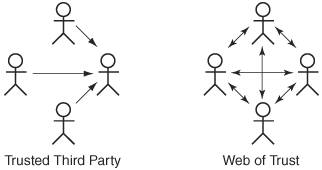
\includegraphics[scale=1.0]{trust_models.jpeg}
\note[itemize]{
\item hierarchies introduce single points of failure
}
\end{frame}

%%%%%%%%%%%%%%%%%%%%%%%%%%%%%%%%%%%%%%%%%%%%%%%%%%%%%%%%%%%%%%%%%%%%%%%%%%%%%%%
\begin{frame}{Web of trust}
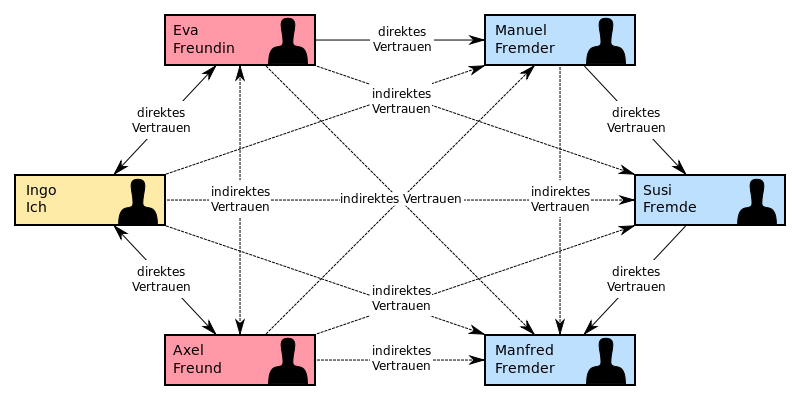
\includegraphics[scale=0.44]{web_of_trust.png}
\note[itemize]{
\item Harder to maintain
\item More resilient
\item Trust is not just boolean, but can be calculated
\item Bank with brass plate with QR code of public key
}
\end{frame}

%%%%%%%%%%%%%%%%%%%%%%%%%%%%%%%%%%%%%%%%%%%%%%%%%%%%%%%%%%%%%%%%%%%%%%%%%%%%%%%
\begin{frame}{NameCoin}
\emph{Namecoin} is a decentralized open source information registration and transfer system based on the Bitcoin cryptocurrency
\begin{itemize}
\item Domain names for .bit TLD
\begin{itemize}
\item Including TLS fingerprint
\end{itemize}
\item Identity information 
\end{itemize}
\\[0.2cm]
\pause
\emph{Zooko's triangle}: properties considered desirable for names of participants in a network protocol
\begin{itemize}
\item \emph{Human-meaningful}: Meaningfulness and memorability to the users
\item \emph{Decentralized}: No need of a centralized authority for determining the meaning of a name
\item \emph{Secure}: There is one, unique and specific entity to which the name applies
\end{itemize}
\\[0.2cm]
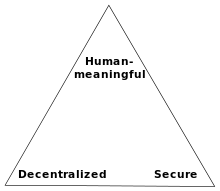
\includegraphics[scale=0.2]{zooko_triangle.png}
\note[itemize]{
\item essentially a secure key value store
\item name and TLS certificate are tied together
\item simple script for dyndns
\item after seeing this it seems strange that you have to buy the name and certificate from different entities with the legacy system
\item I am sure you know the  fast-cheap-complete triangle
}
\end{frame}

%%%%%%%%%%%%%%%%%%%%%%%%%%%%%%%%%%%%%%%%%%%%%%%%%%%%%%%%%%%%%%%%%%%%%%%%%%%%%%%
\begin{frame}{Private key stolen or unintentionally published}
A private key is a very sensitive piece of information, and should be treated accodingly.
\\[0.2cm]
\begin{itemize}
\item Never send a private key over unencrypted eMail % Reto has a story to this
\item Never store a private key unencrypted on a cloud starage
\item A surprising number of private keys were found in github repositories
\item If possible store private keys only on airgapped machines and hardware devices
\item A good example is the YubiKey NEO with an OpenPGP applet
\item If you have to store it on disk, restrict the access rights
\end{itemize}
\end{frame}

%%%%%%%%%%%%%%%%%%%%%%%%%%%%%%%%%%%%%%%%%%%%%%%%%%%%%%%%%%%%%%%%%%%%%%%%%%%%%%%
\begin{frame}{Closing}
All code presented in this document can be found at:\\
\href{https://github.com/ulrichard/experiments/tree/master/trustworthy\textunderscoresoftware}{https://github.com/ulrichard/experiments/tree/master/trustworthy\_software}\\
\\[0.5cm]
It was written using vim, LaTeX and cmake. For more details see:\\
\href{http://blog.ulrichard.ch/?p=1406}{http://blog.ulrichard.ch/?p=1406}\\
\\[0.5cm]
Thanks for listening
\\[0.5cm]
Do you have questions?
\end{frame}

\end{document}

